\newcommand{\ConstExercise}{07}
\newcommand{\ConstDeadline}{26.05.2023}

\documentclass[11pt,letterpaper]{article}
\textwidth 6.5in
\textheight 9.in
\oddsidemargin 0in
\headheight 0in

\usepackage[exp]{custom_0.1}

\begin{document}

%%%%% Document %%%%%

\begin{enumerate}
    \item \textbf{Plattenkondensator im Dielektrikum}
    \begin{enumerate}
        \item
        \begin{align*}
            U &\eq{*} U_1 + U_2\\
            U &= U_1 + \frac{U_1}{\epsilon_r}\\
            U_1 &= \frac{U}{1 + \frac{1}{\epsilon_r}}\\
            U_2 &= U \cbrace{1 - \frac{1}{1 + \frac{1}{\epsilon_r}}}\\
            E_1 &= \frac{U_1}{d_1} \approx \frac{1}{3\,\mathrm{cm}} \frac{200\,\mathrm{V}}{1 + \frac{1}{5}}\approx 5.56\,\ufrac{kV}{m} \\
            E_2 &= \frac{U_2}{d_2} \approx \frac{1}{3\,\mathrm{cm}} 200\,\mathrm{V}\cbrace{1 - \frac{1}{1 + \frac{1}{5}}} \approx 1.11\,\ufrac{kV}{m}
        \end{align*}
        $(*):$ 1 bezeichnet den Teil ohne Dielektrikum, 2 mit Dielektrikum.
        \\
        \item
        Die Länge des mit Luft gefüllten Anteils des Kondensators ist gegeben durch:
        $x_l = x-L$, die des mit Dielektrikum gefüllten Anteils durch: 
        $x_d  = L - x_l = 2L-x$.

        \begin{align*}
            C &= C_1 + C_2\\
            &= \epsilon_0 \frac{A_1}{d} + \epsilon_0\epsilon_r \frac{A_2}{d}\\
            &= \epsilon_0 \frac{x_l b}{d} + \epsilon_0\epsilon_r \frac{x_db}{d}\\
            &= \frac{\epsilon_0 b}{d} \cbrace{x_l + \epsilon_r (L-x_l)}\\
            &= \frac{\epsilon_0 b}{d} \cbrace{x(1 - \epsilon_r ) + L ( 2\epsilon_r - 1)}\\
            \\
            W_U &= \frac{1}{2}C U^2 = \frac{\epsilon_0 b U^2}{2d} \cbrace{x(1 - \epsilon_r ) + L ( 2\epsilon_r - 1)}\\
            F_U &= -\vnabla W_U = -\frac{\epsilon_0 b U^2}{2d}(1 - \epsilon_r ) \\
        \end{align*}
        \begin{align*}
            W_Q &= \frac{1}{2}C \cbrace{\frac{Q}{C}}^2= \frac{1}{2}\frac{Q^2}{C}= \frac{1}{2}\frac{Q^2d}{\epsilon_0 b \cbrace{x(1 - \epsilon_r ) + L ( 2\epsilon_r - 1)}}\\
            F_Q &= -\vnabla W_Q 
            = \frac{1}{2}\frac{Q^2d(1 - \epsilon_r )}{\epsilon_0 b \cbrace{x(1 - \epsilon_r ) + L ( 2\epsilon_r - 1)}^2}
        \end{align*}
    \end{enumerate}

    \item \textbf{Geladener Draht}
    
    Das Koordinaten-System in Zylinderkoordinaten sei so orientiert, dass die z-Achse durch den Draht
    durch geht.

    \begin{align*}
        \vec{E}(\vec{r}) &= E(r)\e_r\\
        \oiint_A \vec{E}(\vec{r})\,\dS
        &= \int_{V}\frac{\rho(\vec{r})}{\epsilon_0} \,\di^3r
        \\
        \int_{0}^{l} \int_{0}^{2\pi}\dA\, E(r)
        &\eq{*} \frac{1}{\epsilon_0} \int_0^l \lambda \,\dz\\
        \int_{0}^{l} \dz\int_{0}^{2\pi}\dphi\,r E(r)
        &= \frac{l \lambda}{\epsilon_0} \\
        2\pi r l E(r) &=  \frac{l \lambda}{\epsilon_0} \\
        E(r) &=  \frac{\lambda}{2\pi \epsilon_0  r} \\
        \vec{E}(\vec{r}) &=  \frac{\lambda}{2\pi \epsilon_0  r} \e_r\\
    \end{align*}
    $(*):$ Für die Stirnflächen eines Zylinders gilt: $\dS \parallel \e_z\implies \dS_{Stirnfl.}\cdot \vec{E}=0$

    \item \textbf{Funkengenerator}
    \begin{align*}
        T_{l}(\ch{Al}) = 933.47 \,\mathrm{K}\quad ,\quad
        c_M(\ch{Al}) = 24.2 \,\ufrac{J}{mol\,K}
    \end{align*}
    \begin{align*}
        W &= \frac{1}{2} C U^2\\
        &\approx \frac{1}{2} \cdot 22000 \,\mathrm{\mu F} \cdot (4\cdot  9\,\mathrm{V})^2\\
        &\approx 14.3 \, \mathrm{J}\\
        \\
        W &= c_M n \Delta T\\ 
        n &= \frac{W}{c_M  (T_l - T_0)}\\ 
         &\approx \frac{14.3 \u{J}}{24.2 \,\ufrac{J}{mol\,K} 
         \cdot(933.47 \,\mathrm{K} - 290 \,\mathrm{K})}\\
         &\approx 9.18 \cdot 10^{-4}\u{mol}= 0.0247 \u{g}
    \end{align*}
\newpage
    \item \textbf{Feldstärke einer Leiterplatte (num.)}
        \begin{enumerate}
            \item
            \begin{align*}
                \sigma &= \frac{Q}{A}
                = \frac{N^2e}{(Nl )^2}
                = \frac{e}{l^2}\\
                e &= \sigma l^2 = 1\ufrac{C}{m^2}\cdot l^2\\
                l &= \sqrt{\frac{e}{\sigma}} =\sqrt{\frac{e}{1\ufrac{C}{m^2}}} 
            \end{align*}

            \item[(b/c)] \ [siehe hinten]\\

            \item [(c)]
            Die numerische Lösung verhält sich mehr wie eine Punktladung, in der Hinsicht, dass 
            die Feldstärke mit steigendem Abstand abfällt, im Gegensatz zur 
            analytischen unendlichen Fläche, die ein konstantes E-Feld hat. 
            Es fällt aber auch auf, dass sich die Propotionalität $E\propto\frac{1}{r^2}$ mit einem 
            höherem $N$ und kleinerem $l$ der Propotionalität der unendlichen Leiterplatte 
            $E\propto 1$ annähert (für kleine $d$).
            
        \end{enumerate}
\end{enumerate}
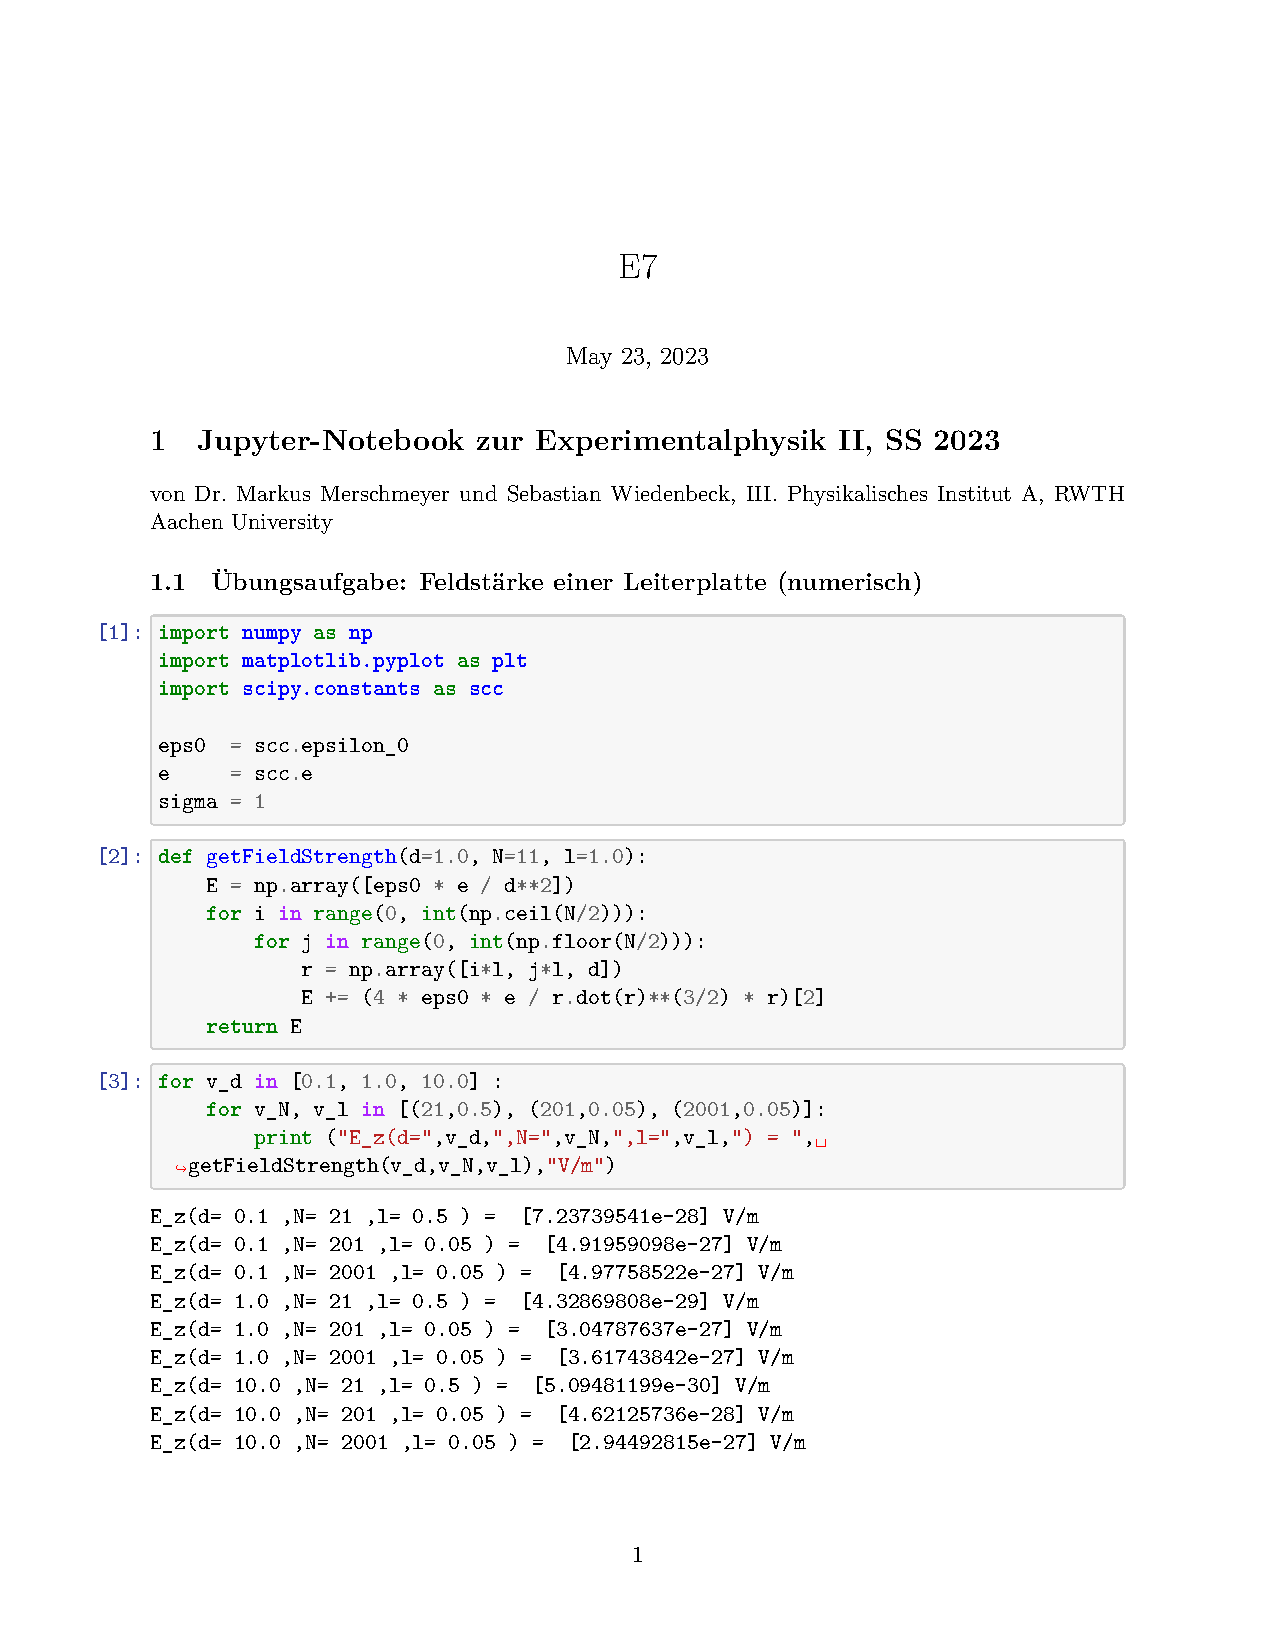
\includepdf{E7.pdf}

\end{document}